% По умолчанию используется шрифт 14 размера. Если нужен 12-й шрифт, уберите опцию [14pt]
\documentclass[14pt
  , russian
  %, xcolor={svgnames}
  ]{matmex-diploma-custom}
 
\usepackage[table]{xcolor}
\usepackage{graphicx}
\usepackage{tabularx}
\newcolumntype{Y}{>{\centering\arraybackslash}X}
\usepackage{amsmath}
\usepackage{amsthm}
\usepackage{amsfonts}
\usepackage{amssymb}
\usepackage{mathtools}
\usepackage{thmtools}
\usepackage{thm-restate}
\usepackage{tikz}
\usepackage{wrapfig}
% \usepackage[kpsewhich,newfloat]{minted}
% \usemintedstyle{vs}
\usepackage[inline]{enumitem}
\usepackage{subcaption}
\usepackage{caption}
\usepackage[nocompress]{cite}
\usepackage{makecell}

\usepackage{multirow}
\usepackage{graphicx}
\usepackage{subcaption}
\usepackage{lscape}
\usepackage{longtable}
\usepackage{tikz}
\usepackage{latexsym}

\usepackage{algpseudocode}
\usepackage{algorithm}
\usepackage{algorithmicx}
\usepackage{verbatim}
\usepackage{mathtools}

\usepackage{subcaption}
\usepackage{colortbl}
\usepackage{balance}

% \setitemize{noitemsep,topsep=0pt,parsep=0pt,partopsep=0pt}
% \setenumerate{noitemsep,topsep=0pt,parsep=0pt,partopsep=0pt}


\graphicspath{ {resources/} }

% 
% % \documentclass 
% %   [ a4paper        % (Predefined, but who knows...)
% %   , draft,         % Show bad things.
% %   , 12pt           % Font size.
% %   , pagesize,      % Writes the paper size at special areas in DVI or
% %                    % PDF file. Recommended for use.
% %   , parskip=half   % Paragraphs: noindent + gap.
% %   , numbers=enddot % Pointed numbers.
% %   , BCOR=5mm       % Binding size correction.
% %   , submission
% %   , copyright
% %   , creativecommons 
% %   ]{eptcs}
% % \providecommand{\event}{ML 2018}  % Name of the event you are submitting to
% % \usepackage{breakurl}             % Not needed if you use pdflatex only.
% 
% \usepackage{underscore}           % Only needed if you use pdflatex.
% 
% \usepackage{booktabs}
% \usepackage{amssymb}
% \usepackage{amsmath}
% \usepackage{mathrsfs}
% \usepackage{mathtools}
% \usepackage{multirow}
% \usepackage{indentfirst}
% \usepackage{verbatim}
% \usepackage{amsmath, amssymb}
% \usepackage{graphicx}
% \usepackage{xcolor}
% \usepackage{url}
% \usepackage{stmaryrd}
% \usepackage{xspace}
% \usepackage{comment}
% \usepackage{wrapfig}
% \usepackage[caption=false]{subfig}
% \usepackage{placeins}
% \usepackage{tabularx}
% \usepackage{ragged2e}
% \usepackage{soul}
\usepackage{csquotes}
% \usepackage{inconsolata}
% 
% \usepackage{polyglossia}   % Babel replacement for XeTeX
%   \setdefaultlanguage[spelling=modern]{russian}
%   \setotherlanguage{english}
% \usepackage{fontspec}    % Provides an automatic and unified interface 
%                          % for loading fonts.
% \usepackage{xunicode}    % Generate Unicode chars from accented glyphs.
% \usepackage{xltxtra}     % "Extras" for LaTeX users of XeTeX.
% \usepackage{xecyr}       % Help with Russian.
% 
% %% Fonts
% \defaultfontfeatures{Mapping=tex-text}
% \setmainfont{CMU Serif}
% \setsansfont{CMU Sans Serif}
% \setmonofont{CMU Typewriter Text}

\usepackage[final]{listings}

\lstdefinelanguage{ocaml}{
keywords={@type, function, fun, let, in, match, with, when, class, type,
nonrec, object, method, of, rec, repeat, until, while, not, do, done, as, val, inherit, and,
new, module, sig, deriving, datatype, struct, if, then, else, open, private, virtual, include, success, failure,
lazy, assert, true, false, end},
sensitive=true,
commentstyle=\small\itshape\ttfamily,
keywordstyle=\ttfamily\bfseries, %\underbar,
identifierstyle=\ttfamily,
basewidth={0.5em,0.5em},
columns=fixed,
fontadjust=true,
literate={->}{{$\to$}}3 {===}{{$\equiv$}}1 {=/=}{{$\not\equiv$}}1 {|>}{{$\triangleright$}}3 {\\/}{{$\vee$}}2 {/\\}{{$\wedge$}}2 {>=}{{$\ge$}}1 {<=}{{$\le$}} 1,
morecomment=[s]{(*}{*)}
}

\lstset{
mathescape=true,
%basicstyle=\small,
identifierstyle=\ttfamily,
keywordstyle=\bfseries,
commentstyle=\scriptsize\rmfamily,
basewidth={0.5em,0.5em},
fontadjust=true,
language=ocaml
}
 
\newcommand{\cd}[1]{\texttt{#1}}
\newcommand{\inbr}[1]{\left<#1\right>}


\newcolumntype{L}[1]{>{\raggedright\let\newline\\\arraybackslash\hspace{0pt}}m{#1}}
\newcolumntype{C}[1]{>{\centering\let\newline\\\arraybackslash\hspace{0pt}}m{#1}}
\newcolumntype{R}[1]{>{\raggedleft\let\newline\\\arraybackslash\hspace{0pt}}m{#1}}



\usepackage{soul}
\usepackage[normalem]{ulem}
%\sout{Hello World}



\begin{document}
%% Если что-то забыли, при компиляции будут ошибки Undefined control sequence \my@title@<что забыли>@ru
%% Если англоязычная титульная страница не нужна, то ее можно просто удалить.
\filltitle{ru}{
    %% Актуально только для курсовых/практик. ВКР защищаются не на кафедре а в ГЭК по направлению, 
    %%   и к моменту защиты вы будете уже не в группе.
    chair              = {Кафедра системного программирования},
    group              = {21.М07-мм},
    %% Макрос filltitle ненавидит пустые строки, поэтому обязателен хотя бы символ комментария на строке
    %% Актуально всем.
    title              = {Разработка библиотеки обобщенной разреженной линейной алгебры для вычислений на GPU},
    % 
    %% Здесь указывается тип работы. Возможные значения:
    %%   coursework - отчёт по курсовой работе;
    %%   practice - отчёт по учебной практике;
    %%   prediploma - отчёт по преддипломной практике;
    %%   practice - отчёт по учебной практике;
    %%   master - ВКР магистра;
    %%   bachelor - ВКР бакалавра.
    type               = {master},
    author             = {Орачев Егор Станиславович},
    % 
    %% Актуально только для ВКР. Указывается код и название направления подготовки. Типичные примеры:
    %%   02.03.03 <<Математическое обеспечение и администрирование информационных систем>>
    %%   02.04.03 <<Математическое обеспечение и администрирование информационных систем>>
    %%   09.03.04 <<Программная инженерия>>
    %%   09.04.04 <<Программная инженерия>>
    %% Те, что с 03 в середине --- бакалавриат, с 04 --- магистратура.
    specialty          = {09.04.04 <<Программная инженерия>>},
    % 
    %% Актуально только для ВКР. Указывается шифр и название образовательной программы. Типичные примеры:
    %%   СВ.5006.2017 <<Математическое обеспечение и администрирование информационных систем>>
    %%   СВ.5162.2020 <<Технологии программирования>>
    %%   СВ.5080.2017 <<Программная инженерия>>
    %%   ВМ.5665.2019 <<Математическое обеспечение и администрирование информационных систем>>
    %%   ВМ.5666.2019 <<Программная инженерия>>
    %% Шифр и название программы можно посмотреть в учебном плане, по которому вы учитесь. 
    %% СВ.* --- бакалавриат, ВМ.* --- магистратура. В конце --- год поступления (не обязательно ваш, если вы были в академе/вылетали).
    programme          = {ВМ.5666.2021 <<Программная инженерия>>},
    % 
    %% Актуально только для ВКР, только для матобеса и только 2017-2018 годов поступления. Указывается профиль подготовки, на котором вы учитесь.
    %% Названия профилей можно найти в учебном плане в списке дисциплин по выбору. На каком именно вы, вам должны были сказать после второго курса (можно уточнить в студотделе).
    %% Вот возможные вариканты:
    %%   Математические основы информатики
    %%   Информационные системы и базы данных
    %%   Параллельное программирование
    %%   Системное программирование
    %%   Технология программирования
    %%   Администрирование информационных систем
    %%   Реинжиниринг программного обеспечения
    % profile            = {Системное программирование},
    % 
    %% Актуально всем.
    supervisorPosition = {Доцент кафедры информатики, к.\,ф.-м.\,н.},
    supervisor         = {С.~В.~Григорьев},
    % 
    %% Актуально только для практик и курсовых. Если консультанта нет, закомментировать или удалить вовсе.
    % consultantPosition = {должность ООО <<Место работы>> степень},
    % consultant         = {К.К. Консультант},
    %
    %% Актуально только для ВКР.
    reviewerPosition   = {Эксперт, ООО "Техкомпания Хуавэй"},
    reviewer           = {С.~В.~Моисеев},
}

\filltitle{en}{
    chair              = {Software Engineering},
    group              = {21.М07-мм},
    title              = {Generalized sparse linear algebra library with vendor-agnostic GPUs accelerated computations},
    type               = {master},
    author             = {Egor Orachev},
    % 
    %% Possible choices:
    %%   02.03.03 <<Software and Administration of Information Systems>>
    %%   02.04.03 <<Software and Administration of Information Systems>>
    %%   09.03.04 <<Software Engineering>>
    %%   09.04.04 <<Software Engineering>>
    %% Те, что с 03 в середине --- бакалавриат, с 04 --- магистратура.
    specialty          = {09.04.04 <<Software Engineering>>},
    % 
    %% Possible choices:
    %%   СВ.5006.2017 <<Software and Administration of Information Systems>>
    %%   СВ.5162.2020 <<Programming Technologies>>
    %%   СВ.5080.2017 <<Software Engineering>>
    %%   ВМ.5665.2019 <<Software and Administration of Information Systems>>
    %%   ВМ.5666.2019 <<Software Engineering>>
    programme          = {СВ.5666.2021 <<Software Engineering>>},
    % 
    %% Possible choices:
    %%   Mathematical Foundations of Informatics
    %%   Information Systems and Databases
    %%   Parallel Programming
    %%   System Programming
    %%   Programming Technology
    %%   Information Systems Administration
    %%   Software Reengineering
    % profile            = {Software Engineering},
    % 
    %% Note that common title translations are:
    %%   кандидат наук --- C.Sc. (NOT Ph.D.)
    %%   доктор ... наук --- Sc.D.
    %%   доцент --- docent (NOT assistant/associate prof.)
    %%   профессор --- prof.
    supervisorPosition = {C.Sc., docent},
    supervisor         = {S.~V.~Grigorev},
    % 
    % consultantPosition = {position at ``Company'', degree if present},
    % consultant         = {C.C. Consultant},
    % %
    reviewerPosition   = {Expert, Huawei},
    reviewer           = {S.~V.~Moiseev},
}
\maketitle
\setcounter{tocdepth}{3}
\tableofcontents

% \begin{abstract}
%   В курсаче не нужен
% \end{abstract}

\section*{Введение}

Все чаще современные системы аналитики и рекомендаций строятся на основе анализа данных, структурированных с использованием \textit{графовой модели}. В данной модели основные сущности представляются вершинами графа, а отношения между сущностями --- ориентированными ребрами с различными метками. Подобная модель позволяет относительно легко и практически в явном виде моделировать сложные иерархические структуры, которые не так просто представить, например, в классической \textit{реляционной модели}. В качестве основных областей применения графовой модели можно выделить следующие: графовые базы данных~\cite{article:querying_graph_databases}, анализ RDF данных~\cite{article:cfpq_and_rdf_analysis}, биоинформатика~\cite{article:rna_prediction} и статический анализ кода~\cite{article:dyck_cfl_code_analysis}.

Поскольку графовая модель используется для моделирования отношений между объектами, при решении прикладных задач возникает необходимость в выявлении более сложных взаимоотношений между объектами. Для этого чаще всего формируются запросы в специализированных программных средствах для управления графовыми базами данных. В качестве запроса можно использовать некоторый \textit{шаблон} на путь в графе, который будет связывать объекты, т.е. выражать взаимосвязь между ними. В качестве такого шаблона можно использовать формальные грамматики, например, регулярные или контекстно-свободные (КС). Используя вычислительно более выразительные грамматики, можно формировать более сложные запросы и выявлять нестандартные и скрытые ранее взаимоотношения между объектами. Например, \textit{same-generation queries}~\cite{inbook:databases_intro}, сходные с сбалансированными скобочными последовательностями Дика, могут быть выражены КС грамматиками, в отличие от регулярных.

Результатом запроса может быть множество пар объектов, между которыми существует путь в графе, удовлетворяющий заданным ограничениям. Также может возвращаться один экземпляр такого пути для каждой пары объектов или итератор всех путей, что зависит от семантики запроса. Поскольку один и тот же запрос может иметь разную семантику, требуются различные программные и алгоритмические средства для его выполнения.  

Запросы с регулярными ограничениями изучены достаточно хорошо, языковая и программная поддержка выполнения подобных запросов присутствует в некоторых в современных графовых базах данных. Однако, полноценная поддержка запросов с КС ограничениями до сих пор не представлена. Существуют алгоритмы~\cite{article:cfpq_and_rdf_analysis, article:hellings_cfpq, inproceedings:matrix_cfpq, inbook:kronecker_cfpq_adbis, article:cfpq_go_for_rdf} для вычисления запросов с КС ограничениями, но потребуется еще время, прежде чем появиться полноценная высокпроизводительная реализация одного из алгоритмов, способная обрабатывать реальные графовые данные.

Работы~\cite{inproceedings:cfpq_matrix_evaluation, inproceedings:cfqp_matrix_with_single_source} в качестве реализации алгоритма~\cite{inproceedings:matrix_cfpq} для выполнения запросов с КС ограничениями с семантикой достижимости и семантикой одного пути показывают, что возможно использовать GPGPU для выполнения наиболее вычислительно сложных частей алгоритма, что дает \textit{существенный} прирост в производительности. 

Недавно представленный алгоритм~\cite{inbook:kronecker_cfpq_adbis} для вычисления запросов с КС ограничениями полагается на операции линейной алгебры: произведение Кронекера (частный случай тензорного произведения), умножение и сложение матриц в полукольце булевой алгебры. Важной задачей является реализация данного алгоритма, так как он в сравнении с~\cite{inproceedings:cfqp_matrix_with_single_source} позволяет выполнять запросы для всех ранее упомянутых семантик, потенциально поддерживает б\'ольшие по размеру КС запросы, с незначительными накладными расходами позволяет выполнять запросы с регулярными ограничениями, а с реализацией на GPGPU позволит получить потенциально приемлемое время выполнения запрсов.
\section{Problem statement}

The goal of this work is the implementation of the generalized sparse linear algebra primitives and operations library with portable vendor-agnostic yet high-performance GPUs accelerated computations. The work can be divided into the following tasks.

\begin{itemize}
    \item Conduct the survey of existing solutions, focusing on design principles and programming model, overview technologies and tools for programming GPU computations and highlight challenges of GPU programming.
    
    \item Develop the architecture of the library. Design the high-level library structure, execution model, storage scheme, GPUs backend for vendor-agnostic and portable computations acceleration.
    
    \item Implement the library according to the developed architecture, including library core, backend for GPUs accelerated computations, some GPU optimizations in order to speedup computations, and a set of common graph algorithms.

    % and a high-level package for library distribution.
    
    \item Conduct the preliminary experimental study of implemented artifacts. Analyse the performance of the proposed solution compared to existing tools, test the portability and scalability of the developed library on GPUs of different device vendors.
\end{itemize}
\section{Обзор предметной области}

Для разработки библиотеки необходимо сперва рассмотреть базовую теорию, а также ознакомиться с существующими подходами к реализации. Для этого предлагается ознакомиться с концепциями, предлагаемыми GraphBLAS, а также рассмотреть существующие инструменты для работы с примитивами разреженной линейной алгебры на GPU, а также те проблемы, которые возникают при программировании подобных решений в GPU-среде. Это поможет обосновать необходимость разработки нового инструмента.

\subsection{Концепции GraphBLAS}

Стандарт GraphBLAS~\cite{paper:graphblas_foundations} представляет математическую нотацию, транслированную в некоторый C API. Данный стандарт оперирует концепциями линейной (разреженной) алгебры. Основные элементы данного стандарта изложены ниже.

\begin{itemize}
    \item \textbf{Примитивы или контейнеры.} Основными контейнерами для хранения данных являются \textit{матрица}, \textit{вектор}, \textit{скаляр} и \textit{маска}. Контейнеры параметризуются типом элементов, которые они хранят. Имеется возможность создания пользовательских типов данных. 
    \item \textbf{Алгебраические структуры.} В качестве основных алгебраических структур используются \textit{полукольцо} и \textit{моноид}. Данные структуры адаптированы для разреженных данных, поэтому они отличаются от тех, которые приняты в алгебре.
    Данные структуры определяют поэлементные функции, которые оперируют данными в контейнерах. Например, эти функции используются в качестве параметров \textit{mult} и \textit{add} при вычислении матричного произведения, где элементы строки и столбца сначала умножаются, а затем некоторым образом суммируются в конечный  элемент. 
    \item \textbf{Операции.} Основными операциями являются произведения матриц и векторов, поэлементные операции, транспонирование, операции свертки, применение масок для фильтрации элементов, а также операции для манипулирования данными.
\end{itemize}

\subsection{Существующие инструменты}

Существующие инструменты для анализа графов в терминах разреженной линейной алгебры можно разделить на две основные категории: специализированные библиотеки и библиотеки примитивов разреженной линейно алгебры (без фокуса на анализ графовых данных). Существующие инструменты используют разные типы вычислителей, включая один или несколько центральных процессоров, или GPU-ускоритель. Далее представленные наиболее популярные и влиятельные из них.

\subsubsection*{SuiteSparse}

Библиотека SuiteSparse~\cite{article:suite_sparse_for_graph_problems} является полной и эталонной реализацией стандарта GpraphBLAS для вычислений на центральном процессоре. Она доступна для использования через упоминаемый ранее GraphBLAS C API для программирования в языковой среде C или C++, а также имеет ряд открытых и поддерживаемых сообществом пакетов, для использования функций библиотеки в других языковых средах, таких как Python через pygraphblas~\cite{net:pygraphblas}. 

В проекте ведется активная работа по поддержке технологии Nvidia Cuda для осуществления вычислений на Nvidia GPU-устройстве, однако информации о поддержке нескольких GPU-устройств в одном вычислителе нет. Кроме этого, также остается открытым вопрос о возможности создания собственных пользовательских типов и функций для вычислений на GPU, поскольку Nvidia Cuda API требует предкомпиляции кода, что на данный момент не предусмотрено в стандарте GraphBLAS.  

\subsubsection*{GraphBLAST}

Библиотека GraphBLAST~\cite{yang2019graphblast} предоставляет примтивы и операции разреженной линейной алгебры для вычислений на GPU-устройстве с использованием технологии Nvidia Cuda. Данная библиотека использует схожие с GraphBLAS концепции, однако она имеет C++ интерфейс и использует обобщенное программирование с использованием Cuda C++ шаблонов для обеспечения возможности создания произвольных пользовательских типов и операций.

Использование подобного API оправдано, так как это упрощает написание прикладных алгоритмов и позволяет использовать компилятор для генерации требуемого вспомогательного кода. Однако существенным недостатком такого подхода является то, что весь код содержится в \textit{заголовочных файлах}, что требует от пользователя постоянное наличие Nvidia NVCC компилятора и полную перекомпиляцию приложения при любых модификациях.

На данный момент проект находится на стадии разработки, и, несмотря на презентацию на тематической конференции, часть функциональности проекта еще недоступна.

\subsubsection*{Cusp}

Библиотека cusp~\cite{net:cusplibrary} предоставляет набор примитивов разреженной линейной алгебры и основных операций для вычислений на центральном процессоре (в однопоточном или параллельном режиме) и на Nvidia GPU-устройстве. Библиотека имеет C++ интерфейс на основе шаблонов, использует обобщенное программирование для параметризации операций. В своей основе она использует библиотеку примитивов для параллельного программирования Nvidia Thrust~\cite{net:cuda_thrust}, которая предоставляет реализацию для таких операций, как \textit{sort}, \textit{reduce}, \textit{gather}, \textit{scan} и т.д. 

Cusp имеет сходный с GraphBLAST интерфейс, однако данная библиотека была спроектирована для произвольных вычислений с использованием линейной алгебры без акцента на графовых данных. Поэтому она не поддерживает ряд важных операций, таких как применение маски или редуцирование значений. 

\subsubsection*{cuBool и SPbLA}

Библиотеки cuBool и SPbLA~\cite{article:spbla} являются попыткой реализации примитивов и операций из стандарта GraphBLAS, но только для булевых значений. Существует множество алгоритмов, которые можно выразить с использованием операций булевой разреженной линейной алгебры,
такие как достижимость в графе с регулярными или контекстно-свободными ограничениями~\cite{inproceedings:cfpq_matrix_evaluation, inbook:kronecker_cfpq_adbis, inproceedings:matrix_cfpq, inproceedings:cfqp_matrix_with_single_source}.

Библиотеки используют Nvidia CUDA и OpenCL API для вычислений на GPU. Кроме этого, библиотека cuBool имеет пакет pycubool~\cite{net:pycubool} для работы в среде Python. Эти библиотеки были разработаны входе подобного исследования в 2021 году. Они могли бы быть взяты как основа в данной работе, однако архитектура решений не позволяет их расширить для использования произвольных типов и пользовательских функций.

\subsubsection*{Общие недостатки}

Далее выделены основные и наиболее важные недостатки представленных решений.

\begin{itemize}
    \item \textbf{Императивный интерфейс.} Стандарт GraphBLAS и многие сходные библиотеки имеют императивный интерфейс, где пользователь явно вызывает одну операцию за другой, используя соответствующие функции. Это существенно усложняет реализацию подобного интерфейса, а также вносит ряд ограничений на оптимизацию и распараллеливание, т.к. библиотека не обладает достаточной информацией о зависимостях между данными, а также о точках синхронизации.
    
    \item \textbf{Использование шаблонов.} Ряд библиотек, которые реализуют GraphBLAS в виде C++ API, используют шаблоны языка для обобщенного программирования примитивов и операций. Это снижает количество вспомогательного кода, однако делает невозможным единовременную компиляцию такой библиотеки и ее распространение для конечных пользователей без требования локальной компиляции. 
    
    \item \textbf{Использование Nvidia CUDA.} Библиотеки, использующие GPU-устройство для ускорения вычислений, полагаются чаще всего на Nvidia Cuda C++ API, так как оно имеет удобный механизм шаблонов. Однако Cuda технология поддерживается только на графических картах компании Nvidia, что существенно снижает количество потенциальных компьютеров для вычислений.
\end{itemize}

\subsection{Вычисления на GPU-устройстве}

\textit{GPGPU} (от англ. general-purpose computing on graphics processing units) --- техника использования графического процессора видеокарты компьютера для осуществления неспециализированных вычислений, которые обычно проводит центральный процессор. Данная техника позволяет получить значительный прирост производительности, когда необходимо обрабатывать большие массивы однородных данных фиксированным набором команд. 

Термин \textit{multi-GPU} (от англ. multiple GPUs) используется для обозначения вычислительной инфраструктуры, в которой доступно несколько GPU-устройств. Приложения, созданные для подобной среды, автоматически осуществляют распределение вычислений по всем доступным устройствам. 

Существует несколько промышленных стандартов для создания программ, использующих графический процессор, одними из которых являются Vulkan~\cite{net:spec_vulkan}, OpenGL~\cite{net:spec_opengl}, DirectX~\cite{net:spec_direct3d} как API для графических и неспециализированных вычислительных задач, а также OpenCL~\cite{net:spec_opencl}, Nvidia Cuda~\cite{net:cuda_toolkit_docs} как API для неспециализированных вычислений. 

В существующих графовых инструментах основными технологиями для распараллеливания вычислений на графических устройствах являются OpenCL и Nvidia Cuda. Далее представлен краткий обзор каждой из технологий.

\begin{itemize}
    \item \textbf{Nvida Cuda API} является проприетарной технологией компании Nvidia и доступен только на графических устройствах этой компании. Данный API имеет языковую поддержку как С так C++ возможностей, позволяет использовать шаблоны для обобщенного программирования, что упрощает разработку множества алгоритмов, таких как \textit{sort}, \textit{scan}, \textit{reduce}, которые параметризуются типами элементов и операциями. Кроме того, компания Nvidia поставляет множество инструментов для отладки и профилирования Cuda-кода. Также Nvidia Cuda имеет средства для multi-GPU программирования.
    
    \item \textbf{OpenCL API} это открытый стандарт для создания программ, использующих различного типа ускорители для распараллеливания вычислений. Данный стандарт имеет поддержку на множестве платформ, включая Intel, Nvidia, AMD, Apple M1, что делает его применимым на широком классе устройств. Данный API спроектирован в виде C-интерфейса, он не имеет встроенной поддержки для осуществления обобщенного программирования, как в Cuda C++. Также OpenCL имеет средства для multi-GPU программирования. Так как данный стандарт является открытым, на разных платформах качество его поддержки, а также актуальная версия отличаются, что делает проблематичным разработку и отладку OpenCL-приложений.
\end{itemize}

В данной работе в качестве технологии для программирования GPU-вычислений используется OpenCL. Данный API выбран, поскольку его требуемая версия 1.2 для проекта имеет поддержку на всех актуальных устройствах. Также данный API позволяет динамически во время исполнения компилировать код для выполнения на GPU, что делает его удобным инструментов для создания \textit{обобщенной} библиотеки, где пользователь сможет реализовывать свои примитивные типы и операции в виде набора текстовых строк.

% \subsection{Алгоритмы разреженной линейной алгебры для GPU}
\section{Архитектура библиотеки}

\subsection{Структура}

Архитектура библиотеки представлена на рис.~\ref{fig:cubool_architecture}.
Структура библиотеки и ее конечначная функциональность в основном продиктованы следующими высокоуровневыми требованиями, которые продиктованы как конечными вычислительными задачами на GPGPU, так и наличием существующей инфраструктуры для осуществления экспериментов~\cite{net:cfpq_py_algo}.

\begin{itemize}
    \item Поддержка вычислений на Cuda-девайсе.
    \item Поддержка вычислений на CPU.
    \item C-совместимое API для работы с библиотекой.
    \item Python-пакет для работы с примитивами и операциями библиотеки в управляемой высокоуровневой стреде языка Python.
    \item Поддержка логирования, функций для отладки и протопирования конечных пользовательских алгоритмов.
\end{itemize}

\begin{figure}[h]
    \centering
    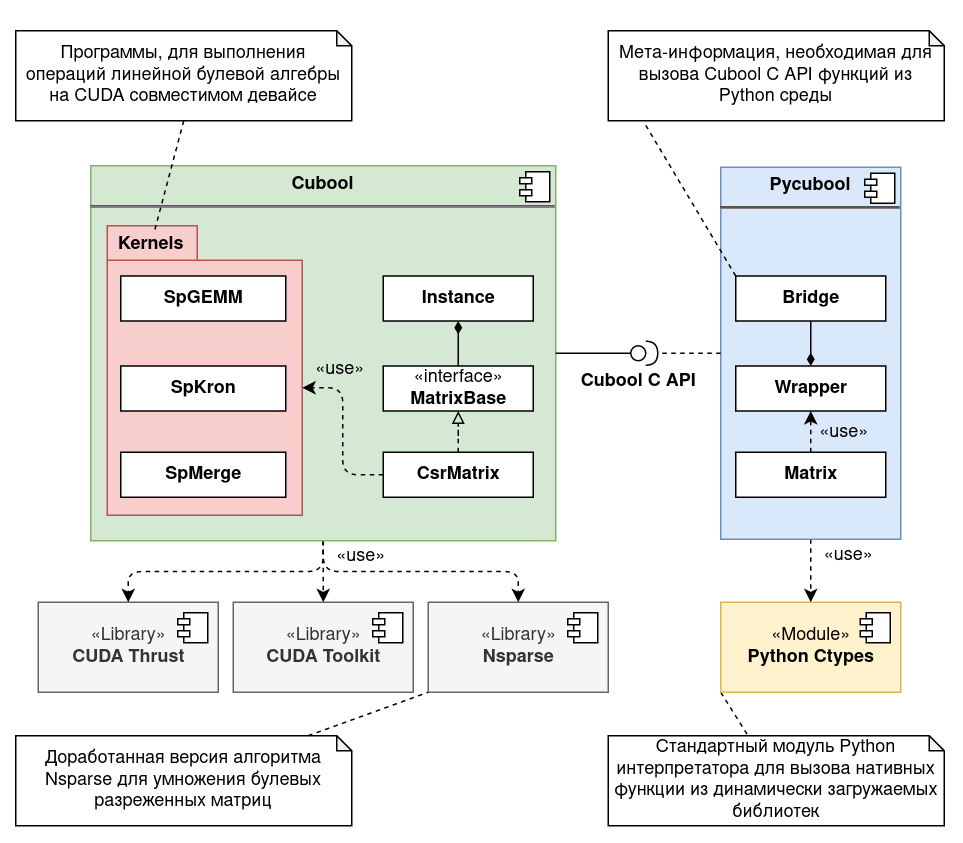
\includegraphics[width=0.8\textwidth]{images/library_architecture.png}
    \caption{Архитектура разработанной библиотеки}
    \label{fig:cubool_architecture}
\end{figure}

\subsection*{Core}

Класс \textbf{Library} поддерживает глобальное состояние библиотеки, осуществляет конфигурацию и инициализацию, выбор конкретного вычислительного бэкенда, первичную валидацию вызовов функций и входных данных пользователя, 
а также осуществляет хранение всех созданых объектов. 

Класс \textbf{Matrix} является proxy-классом, который осуществяет доступ к операциям конкретного вычислительного бэкенда, которой был выбран пользователем на этапе инициализации всей библиотеки.
Данный подход позволяет не только динамически выбирать платформу вычислений, 
но также позволяет осуществлять дополнительную обработку ошибок, 
а также поддерживать дополнительные операции над матрицами.

Класс \textbf{Logger} осуществляет логгирование в выбранный пользователем текстовый файл в процессе использования функций библиотеки, а также позволяет профилировать операций и также сохранять время их выполенения в текстовом виде.

\subsection*{Backend}

Интерфейс \textbf{MatrixBase} предоставляет набор основных функций и операций, которые каждый вычислительный бэкенд должен реализовывать для того, чтобы эти матрицы можно было использовать в \textbf{Core} непосредственно для вычислений.

Интерфейс \textbf{BackendBase} описывает базовый контракт, которой должен предоставлять вычислительный бэкенд. Данный интерфейс включает в себя функции для создания и удаления матриц, спефичных для этого буэкенда, а также функции для корректной инициализации и завершения работы данного бэкенда.

\subsection*{Cuda}

Класс \textbf{CudaMatrix} реализует интерфейс \textbf{MatrixBase} и предоставляет операции, для работы с матрицами и осуществления вычислений на Cuda-девайсе. \textbf{CudaMatrix} поддерживает данные матрицы (не нулевые элементы) в видео-памяти, и использует Cuda \textit{kernels} для осуществления вычислений на GPU. \textit{Kernels} хранятся в виде функций вместе с исходным кодом модуля.

Данный вычислительный бэкенл выбирается по умолчанию, если в компьтере пользователся имеется Cuda-девайс.
Однако пользователь может в таком случае все равно может выбрать \textbf{Sequent} вычисления. 

\subsection*{Sequent}

Предоставляет реализацию класса матрицы и операций над ней для вычислений на CPU. Все вычислений осуществляются последовательно, в однопоточном режиме, не требуют дополнительных библиотек или компонентов.

Данных вычислительный бэкенд используется по умолчанию на устройствах без Cuda-девайса. Данный подход позволит использовать библиотеку всем пользователям без исключения. Также данный подход может быть удобен для прототипирования алгоритмов на локальном компьютере, чтобы позже запустить вычисления на высокопроизводительном сервере с поддержкой Cuda.

\subsection*{Pycubool}

Python-пакет предоставляет доступ к примитивам и операциям библиотеки в языковой среде Python.
Модуль \textbf{matrix} предоставляет доступ к классу матрицы и основным операциям, дотсупным в C API.
Модуль \textbf{bridge} осуществляет коммуникацию с библиотекой через механизмы вызова нативных методов. Модуль \textbf{wrapper} поддерживает глобальное состояние библиотеки в во время работы Python-интерпретатора. Модули \textit{io} и \textbf{gviz} предоставляют доступ к операциям ввода/вывода данных, позволяют загружать или сохранять матрциы в виде текстовых на диск, а также экспортировать набор матриц в виде графа в формате GraphViz, что может быть полезно для отладки алгоритмов.

\subsection{Последовательнось обработки операций}

На рис.~\ref{fig:cubool_sequence} представлена последовательность обработки вычислительной операции над матрицей (матрицами) на Cuda-девайсе. 

Пользовательский Python-код инициирует выполнение операции над мамтрицей или несколькими матрицами внутри инфраструктуры Python. Этот вызов обрабатывает \textbf{pycubool}-пакет, который осуществляет первичную базовую валидацию аргументом, осуществляет их запаковку и передачу в нативную функцию \textbf{cuBool C API}. На стороне реализации данного интерфейса, полученные аргументы приводятся к требуемому типу и передаются далее в модуль \textbf{Core}, который поддерживает состояние библиотеки, осуществяет валидацию аргументов, а также определяет допустимость выполнения операции. Далее вызов передается непосредственно вычислительному бэкенду \textbf{Cuda}, который осуществляет подготовку и непосредственный запуск вычислений на сороне \textbf{Nvidia GPU}. 

Когда вычисление завершается, \textbf{Cuda}-бэкенд обновляет состояние матриц в соответсвии с полученными результами. Модуль \textbf{Core} осуществяет финальное логирование операции, а также сохраняет временные показатели выполнения вычислений в файл (опционально), и возвращает в качестве результата выполнения статус операции, либо возможное исклбчение, которое могло возникнуть на этапе обработки запроса вычислений. \textbf{cuBool C API} осуществяет финальную обработку исключения (если таковое возникло), и возвращет вызываещему числовой идентефикатор статуса операции. 

В результате выполнения операции \textbf{pucubool} уведомляет пользователя о потенциально возникших ошибках и возвращает управление из вызываемой функции. Обновленное состояние библиотеки находится в \textbf{Core}, а состояние матриц после выполнения операций хранится на стороне \textbf{Cuda}-бэкенда. 

\begin{figure}[h]
    \centering
    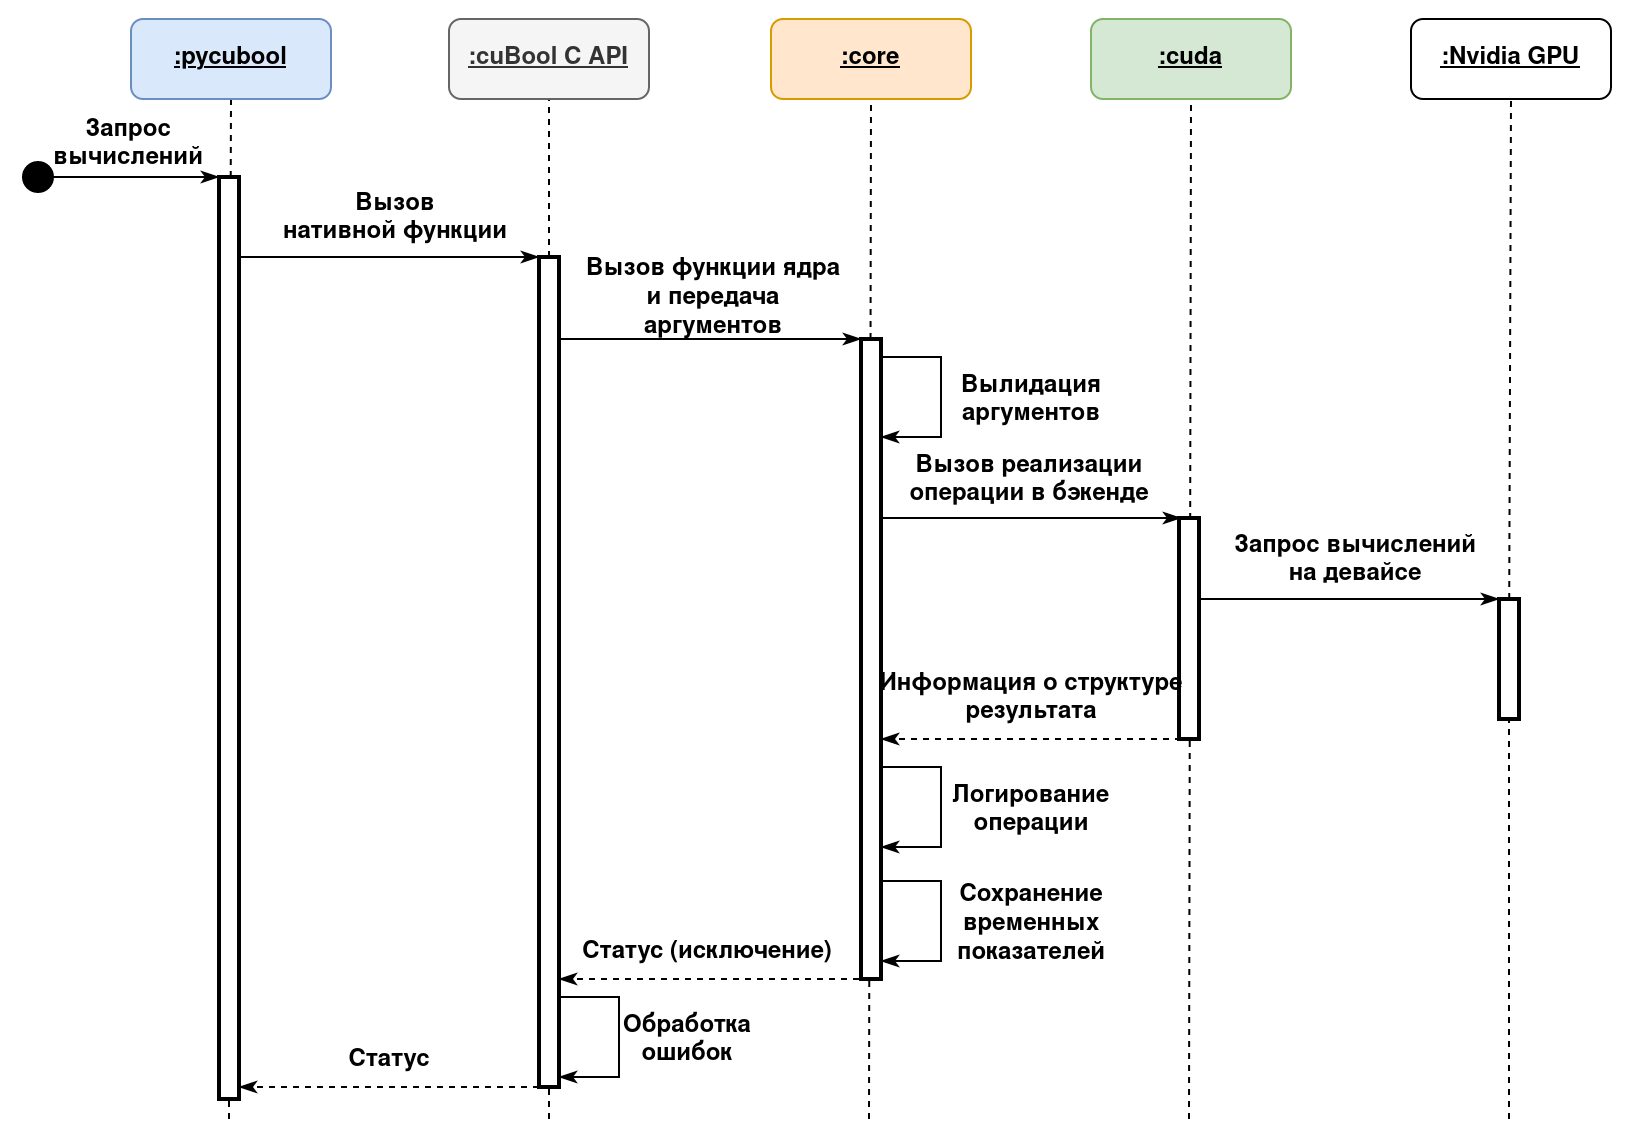
\includegraphics[width=0.8\textwidth]{images/library_sequence_use.png}
    \caption{Последовательность обработки вызова вычислительной матричной операции на Nvidia GPU}
    \label{fig:cubool_sequence}
\end{figure}



\section{Детали реализации}

В данной секции изложены основные детали реализации библиотеки \textit{cuBool} и соответствующего ей Python-пакета \textit{pycubool}.

Разработка библиотеки осуществлялась в рамках исследовательского проекта лаборатории языковых инструментов JetBrains Research. В качестве языка программирования для реализации библиотеки используется С++, 
так как он предоставляет механизмы для ручного управления ресурсами, 
а также позволяет использовать язык Cuda C/C++ в рамках единого компилируемого приложения. 
Интерфейс библиотеки реализован в виде C-совместимого API.
Исходный код компилируется в библиотеку с разделяемым кодом \textbf{libcubool.so}, 
которая может быть динамически загружена в конечное пользовательское приложение. 
В качестве целевой платформы для исполнения поддерживается семейство операционных систем на базе ядра Linux.

\subsection{Примитивы и операции}

Основным примитивом библиотеки является разреженная матрица булевых значений, 
которая хранится в видеопамяти видеокарты в формате \textit{CSR} (compressed sparse row), 
который позволяет использовать $O(V + E)$ памяти для хранения матрицы смежности графа. 
Существуют и другие форматы хранения разреженных матриц: \textit{CSC} (compressed sparse column), \textit{COO} (coordinate list) и так далее. 
Однако CSR формат был выбран на основе результатов исследования Юсуке Нагасака и др.~\cite{inproceedings:spgemm_mem_saving_for_nvidia}, 
так как он позволяет эффективно реализовать операцию матричного умножения в условиях ограниченного объема доступной видеопамяти. 

В качестве поэлементных операций сложения и умножения используются \textit{логическое-или} и \textit{логическое-и}. 
Основные функции работы с матрицами представлены ниже.

\begin{itemize}[noitemsep,topsep=0pt,parsep=0pt,partopsep=0pt]
    \item Создание матрицы $M$ размера $m \times n$.
    \item Удаление матрицы $M$ и освобождение занятых ею ресурсов.
    \item Заполнение матрицы $M$ списком значений $\{(i, j)_k\}_k$.
    \item Чтение из матрицы $M$ списка значений $\{(i, j)~|~M[i,j]=1\}$.
    \item Транспонирование матрицы $M = N^T$.
    \item Извлечение подматрицы $M = N[i:k, j:t]$.
    \item Редуцирование матрицы к вектору $V$:~$V[i]=\bigcup_j M[i,j]$.
    \item Сложение матриц $C \mathrel{+}= M$.
    \item Умножение матриц $C \mathrel{+}= M \times N$.
    \item Произведение Кронекера для двух матриц $C = M \otimes N$.
\end{itemize}

\subsection{Cuda-модуль}

Операции линейной алгебры для работы с матрицами реализованы с использованием технологии Cuda. 
В качестве основы для реализации операций умножения и сложения разреженных матриц используются результаты исследования Арсения Терехова и др.~\cite{inproceedings:cfqp_matrix_with_single_source}, оформленные в виде библиотеки \textbf{Nsparse}.
Данная библиотека была доработана, чтобы добавить возможность динамически конфигурировать механизмы использования видеопамяти. 

Для реализации произведения Кронекера, операций транспонирования, редуцирования и извлечения подматрицы использовались примитивы библиотеки \textbf{Thrust}.
Данная библиотека позволяет оперировать данными в терминах высокоуровневых операций \textit{свертки}, \textit{отображения} и \textit{префиксной суммы}~\cite{net:cuda_thrust}, которые выполняются на графическом процессоре. 
\textbf{Thrust} поставляется совместно с инструментами Cuda-разработки и не требует настройки дополнительных зависимостей.

\subsection{Python-пакет}

Все примитивы и операции библиотеки cuBool доступны внутри Python-пакета pycubool.
Для публикации пакета используется стандартная инфраструктура PyPI.
Вызов функций из \textbf{cuBool C API}, находящихся в скомпилированной библиотеке \textbf{libcubool.so}, осуществляется с помощью модуля \textbf{Ctypes}. 
Данный модуль поставляется вместе с инфраструктурой Python и не требует настройки сторонних зависимостей. 
Также в пакет pycubool добавлены дополнительные операции, которые облегчают использование данного инструмента и предоставляют конечному пользователю дополнительную функциональность.

\begin{itemize}[noitemsep,topsep=0pt,parsep=0pt,partopsep=0pt]
    \item Загрузка и сохранение матрицы в \textit{Matrix market} формате.
    \item Экспортирование набора матриц в \textit{GraphViz} формате.
    \item \textit{Красивая} печать матриц в текстовом виде.
    \item Текстовые маркеры и имена матриц для отладки.
\end{itemize}

\subsection{Пример использования}

\definecolor{codegreen}{rgb}{0,0.6,0}
\definecolor{codegray}{rgb}{0.5,0.5,0.5}
\definecolor{codepurple}{rgb}{0.58,0,0.82}
\definecolor{backcolour}{rgb}{1.0,1.0,1.0}

\lstdefinestyle{codelistingstyle}{
    backgroundcolor=\color{backcolour},   
    commentstyle=\color{codegreen},
    keywordstyle=\color{magenta},
    numberstyle=\tiny\color{codegray},
    stringstyle=\color{codepurple},
    basicstyle=\ttfamily\footnotesize,
    breakatwhitespace=false,         
    breaklines=true,                 
    captionpos=b,                    
    keepspaces=true,                 
    numbers=left,                    
    numbersep=5pt,                  
    showspaces=false,                
    showstringspaces=false,
    showtabs=false,                  
    tabsize=2
}

\lstset{style=codelistingstyle}

\begin{algorithm}[]
\floatname{algorithm}{Listing}
\caption{Пример вычисления транзитивного замыкания с использованием cuBool C API}
\label{alg:cubool_example}
\begin{lstlisting}[language=C++]
#include <cubool/cubool.h>

cuBool_Status TransitiveClosure(cuBool_Matrix A, cuBool_Matrix* T) {
    cuBool_Matrix_Duplicate(A, T);                       /* Копируем матрицу смежности А */

    cuBool_Index total = 0;
    cuBool_Index current;
    cuBool_Matrix_Nvals(*T, &current);                   /* Количество ненулевых значений */

    while (current != total) {                           /* Пока результат меняется  */
        total = current;
        cuBool_MxM(*T, *T, *T, CUBOOL_HINT_ACCUMULATE);  /* T += T x T */
        cuBool_Matrix_Nvals(*T, &current);
    }

    return CUBOOL_STATUS_SUCCESS;
}
\end{lstlisting}
\end{algorithm}

\begin{algorithm}[]
\floatname{algorithm}{Listing}
\caption{Пример вычисления транзитивного замыкания с использованием пакета pycubool}
\label{alg:pycubool_example}
\begin{lstlisting}[language=Python]
import pycubool

def transitive_closure(a: pycubool.Matrix):
    t = a.duplicate()                     # Копируем матрицу смежности А
    total = 0                             # Количество ненулевых значений результата

    while total != t.nvals:               # Пока результат меняется
        total = t.nvals
        t.mxm(t, out=t, accumulate=True)  # t += t x t

    return t
\end{lstlisting}
\end{algorithm}

В качестве примера рассмотрим проблему вычисления \textit{транзитивного замыкания} (англ. transitive closure) для некоторого ориентированного графа без меток $\mathcal{G} = \langle V, E \rangle$. Результатом вычисления транзитивного замыкания является новый граф $\mathcal{G}_{tc} = \langle V, E_{tc} \rangle$, для которого верно следующее: $e = (v,u) \in E_{tc} \iff \exists v \pi u $ в $\mathcal{G}$. Данную проблему можно решить в терминах линейной алгебры, если представить граф в виде матрицы смежности с булевыми значениями. 

В листинге~\ref{alg:cubool_example} представлен фрагмент кода на языке C, который решает данную задачу. В качестве аргументов функция принимает матрицу смежности исходного графа, а также указатель на идентификатор, который необходимо использовать при сохранении результирующей матрицы смежности графа после транзитивного замыкания.

В листинге~\ref{alg:pycubool_example} представлен похожий фрагмент кода, однако он уже решает поставленную в задачу на языке Python. Здесь в качестве входного аргумента используется матрица смежности графа, в качестве результата возвращается матрица смежности графа после транзитивного замыкания.

\section{Алгоритм поиска путей с КС ограничениями через тензорное произведение на GPGPU}

% \subsection{Инфраструктура вычислений}

% \subsection{Формат представления данных}

% \subsection{Детали реализации}
\section{Evaluation}

For performance analysis of the proposed solution, a few most common graph algorithms were evaluated using real-world sparse matrix data. 
The following tools for comparison were chosen: LaGraph~\cite{misc:la_graph}~(ver. Feb 13, 2022) in connection with SuiteSparse~\cite{article:suite_sparse_for_graph_problems}~(ver. Jan 14, 2022) as a baseline CPU tool, Gunrock~\cite{article:gunrock}~(ver. Nov 7, 2021) and GraphBLAST~\cite{yang2019graphblast}~(ver. Jun 18, 2021) as a Nvidia GPU tools. 
Also, algorithms were tested on several devices with distinct OpenCL vendors in order to validate the portability of the proposed solution. 

\subsection{Research questions}

In general, these evaluation intentions are summarized in the following research questions. 

\vspace{0.2cm}
\begin{itemize}
    \item[\textbf{RQ1}] What is the performance of the proposed solution relative to existing tools for GPU analysis?

    \item[\textbf{RQ2}] What is the performance of the proposed solution on various devices vendors and OpenCL runtimes?

    \item[\textbf{RQ3}] What is the performance of the proposed solution on integrated GPU compared to existing CPU tool for analysis?
\end{itemize}

\subsection{Evaluation setup}

\textbf{For evaluation of RQ1}, a PC with Ubuntu 20.04 installed used, which has 3.40Hz Intel Core i7-6700 4-core CPU, DDR4 64Gb RAM, Intel HD Graphics 530 integrated GPU, and Nvidia GeForce GTX 1070 dedicated GPU with 8Gb on-board VRAM. 

\textbf{For evaluation of RQ2}, a PC with Ubuntu 22.04 installed used, which has 4.70Hz AMD Ryzen 9 7900x 12-core CPU, DDR4 128 GB RAM, AMD GFX1036 integrated GPU, and either Intel Arc A770 flux dedicated GPU with 8GB on-board VRAM or AMD Radeon Vega Frontier Edition dedicated GPU with 16GB on-board VRAM.

\textbf{For evaluation of RQ3}, the first PC with Intel CPU and integrated GPU and the second PC with AMD CPU and integrated GPU are used.

Spla and LaGraph were compiled with GCC v9.4. Gunrock and GraphBLAST were compiled with GCC v8.4 and Nvidia NVCC v10.1.
Release mode and maximum optimizations level were enabled for all tested programs. 

\subsection{Methodology}

All tests are averaged across 10 runs. The deviation of measurements does not exceed the threshold of 10 percent. Additional warm-up run for each test execution is excluded from measurements. 

Only actual execution time of algorithms is measured. Data loading time, preparation, format transformations, and host-device initial communications are excluded from time measurements. 

The graph vertex with index 1 is set as the initial traversal vertex in the algorithms BFS and SSSP for all tested instruments and all tested devices.

For measurements standard official benchmarks are used, which provided by compared tools developers. These benchmarks are intended for performance comparison. Thus, all tools agree on measurements, what is clearly seen from the source code of those benchmarks.

\subsection{Graph algorithms}

For preliminary study \textit{breadth-first search} (BFS), \textit{single-source shortest paths} (SSSP), \textit{page rank} (PR) and \textit{triangles counting} (TC) algorithms were chosen.
Implementation of those algorithms for competitors is used from official source code repositories with default parameters. Compared tools are allowed to make any optimizations as long as the result remains correct.

\subsection{Dataset}

\begin{table}[tbp]
\caption{Dataset description.} 
\begin{center}
    \begin{tabular}{|l|r|r|r|r|r|}
    \hline
    \multirow{2}{*}{Graph} & \multirow{2}{*}{Vertices} & \multirow{2}{*}{Edges} & \multicolumn{3}{c|}{Out Degree} \\ 
    \cline{4-6} & & & \multicolumn{1}{r|}{Avg} & \multicolumn{1}{r|}{Sd} & \multicolumn{1}{r|}{Max} \\
    \hline
    \hline
    \rowcolor{black!10} coAuthorsCit&227.3K&1.6M&7.2&10.6&1.4K\\
    \rowcolor{black!2 } coPapersDBLP&540.5K&30.5M&56.4&66.2&3.3K\\
    \rowcolor{black!10} amazon2008&735.3K&7.0M&9.6&7.6&1.1K\\
    \rowcolor{black!2 } hollywood2009&1.1M&112.8M&98.9&271.9&11.5K\\
    \rowcolor{black!10} comOrkut&3.1M&234.4M&76.3&154.8&33.3K\\
    \rowcolor{black!2 } citPatents&3.8M&33.0M&8.8&10.5&793.0\\
    \rowcolor{black!10} socLiveJournal&4.8M&85.7M&17.7&52.0&20.3K\\
    \rowcolor{black!2 } indochina2004&7.4M&302.0M&40.7&329.6&256.4K\\
    \hline
    \rowcolor{black!10} belgiumosm&1.4M&3.1M&2.2&0.5&10.0\\
    \rowcolor{black!2 } roadNetCA&2.0M&5.5M&2.8&1.0&12.0\\
    \rowcolor{black!10} rggn222s0&4.2M&60.7M&14.5&3.8&36.0\\
    \rowcolor{black!2 } rggn223s0&8.4M&127.0M&15.1&3.9&40.0\\
    \rowcolor{black!10} roadcentral&14.1M&33.9M&2.4&0.9&8.0\\
    \hline
    \end{tabular}
    \label{dataset:info}
\end{center}
\end{table}

Thirteen matrices with graph data were selected from the Sparse Matrix Collection at University of Florida~\cite{dataset:sparse_matrix_collection}. Information about graphs is summarized in Table~\ref{dataset:info}. This is a common graphs collection used for sparse linear algebra and graph algorithms benchmarks in other works in the domain. These graphs represents typical analysed data structure, sparsity, distribution, and allows one to study common behaviour and performance characteristics of developed libraries.

The dataset is converted to undirected graphs. Self-loops and duplicated edges are removed. Average, sd and max metrics relate to out degree property of the vertices. For SSSP weights are initialized using pseudo-random generator with uniform $[0, 1]$ distribution of floating-point values.

Graphs are roughly divided into two groups. The first group represents relatively dense graphs, where the number of edges per node is sufficient on average to effectively load the GPU with useful work. The second group represents relatively sparse graphs, where the average vertex degree is below the typical GPU vector register size, and the search depth reaches hundreds of hoops. Graphs are sorted in ascending order by the number of vertices within each group.

\subsection{Results Summary}

\begin{figure*}[tbp]
\centering
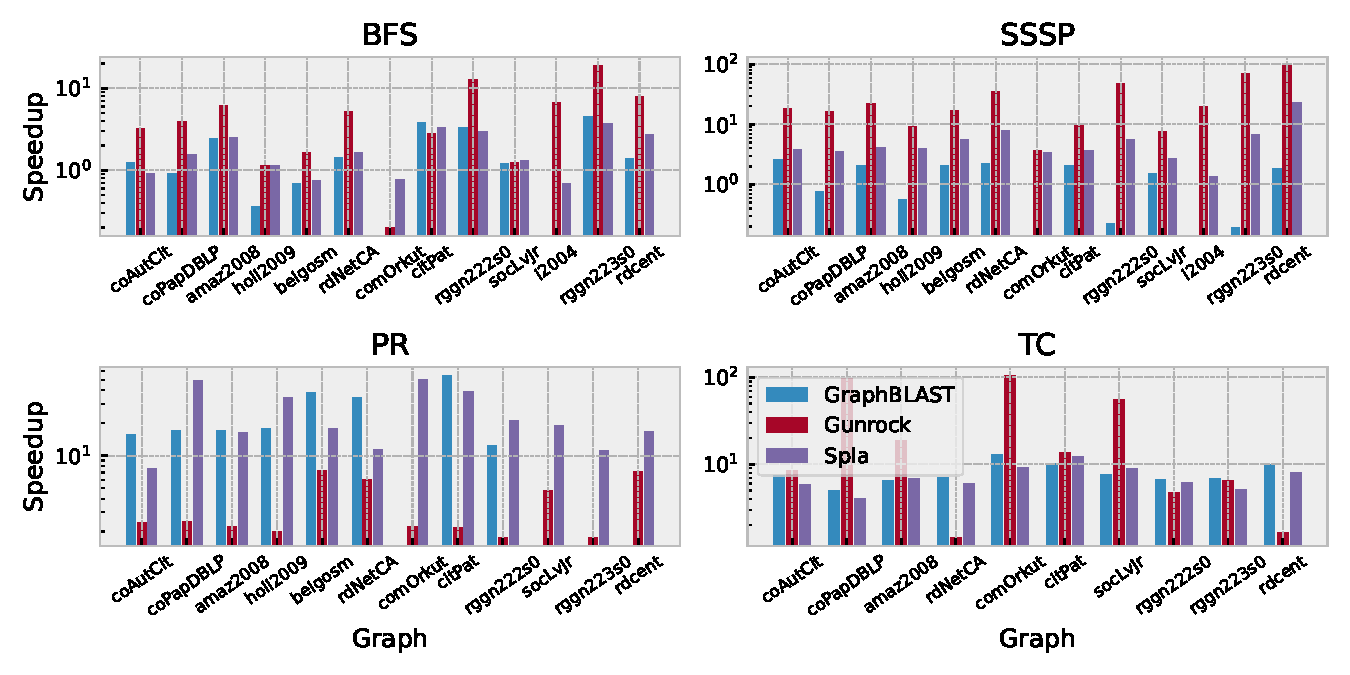
\includegraphics[width=1.0\linewidth]{plots/rq1_rel.pdf}
\caption{Performance of Spla library and GPU tools on the same device compared to LaGraph. Logarithmic scale is used.}
\label{fig:rq1_chart}
\end{figure*}

\begin{figure*}[tbp]
\centering
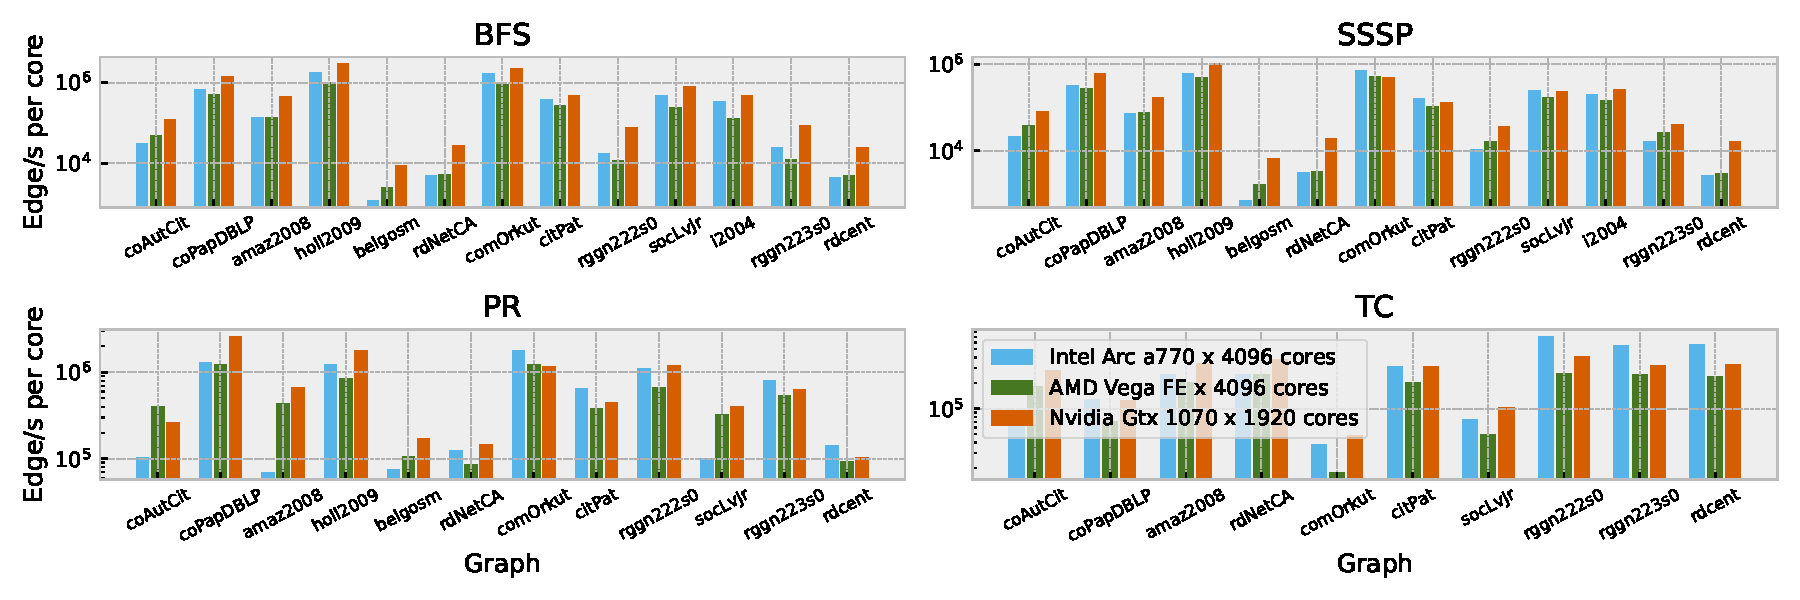
\includegraphics[width=1.0\linewidth]{plots/rq2_cores.pdf}
\caption{Performance of Spla library on different devices relative to the number of compute cores. Logarithmic scale is used.}
\label{fig:rq2_chart}
\end{figure*}

\begin{figure*}[tbp]
\centering
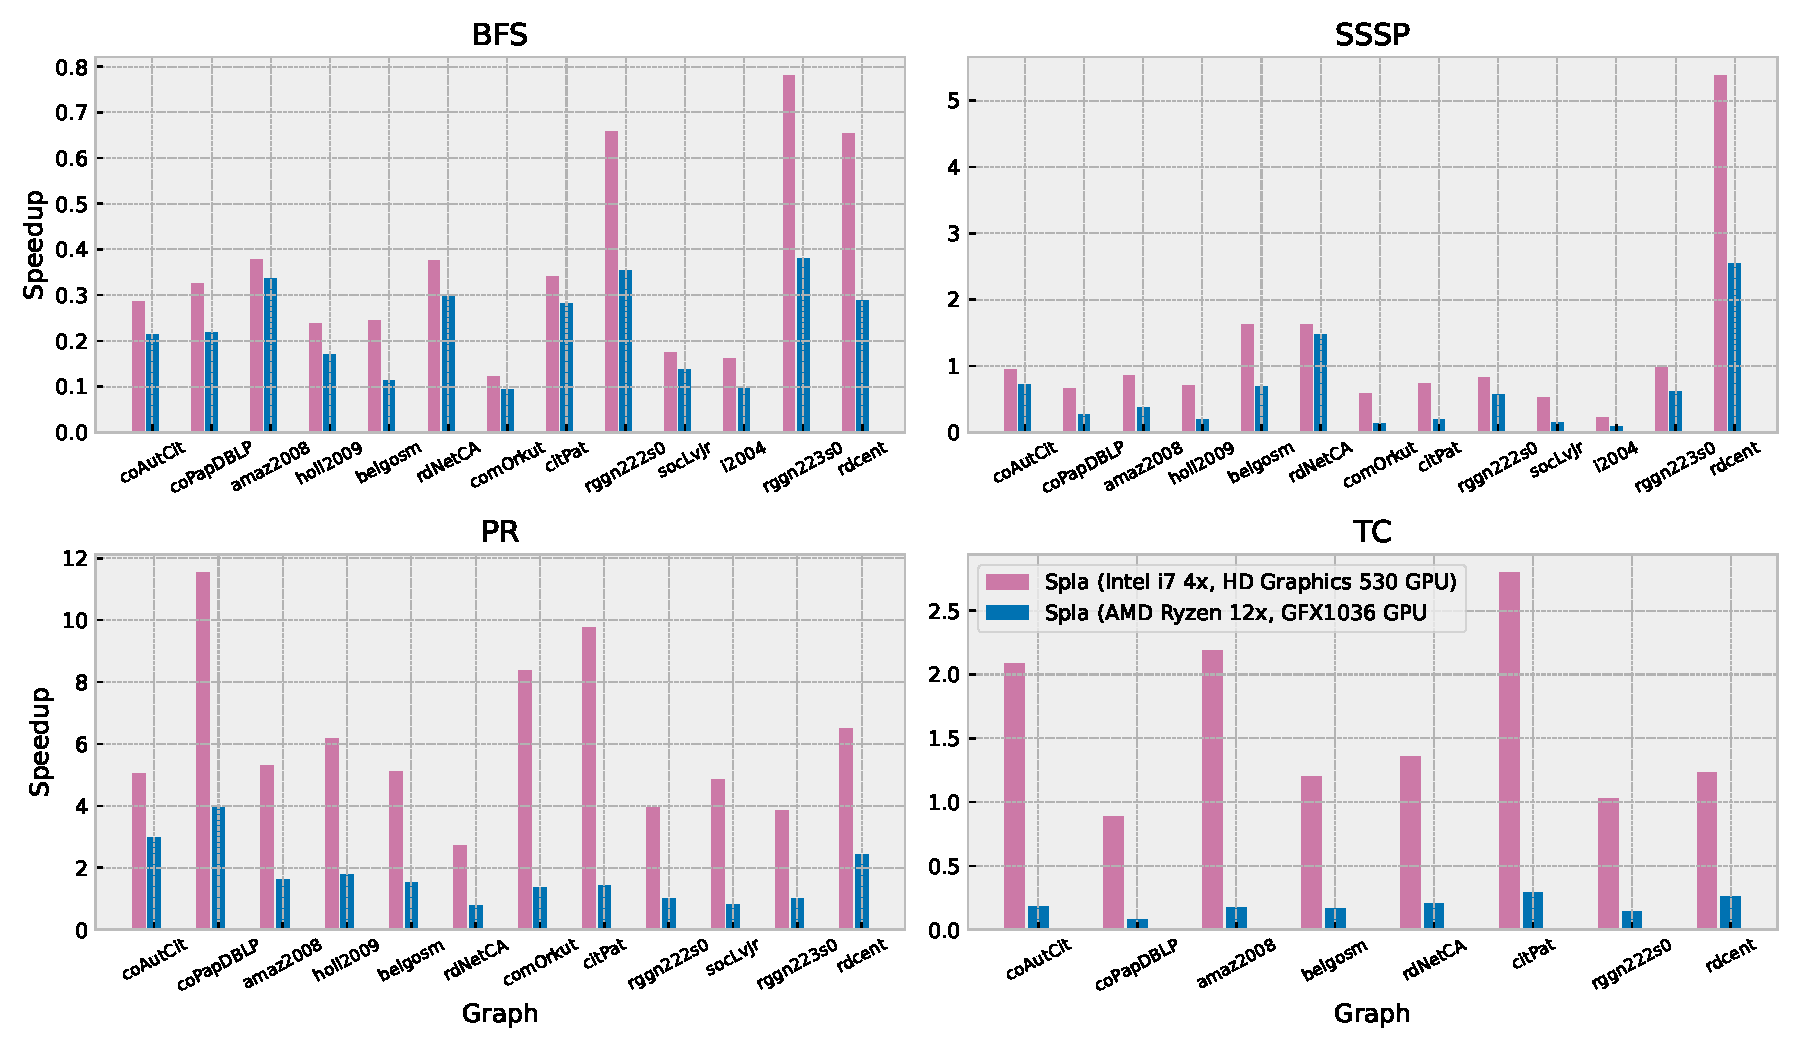
\includegraphics[width=1.0\linewidth]{plots/rq3_int.pdf}
\caption{Performance of Spla library on integrated GPU compared to LaGraph on the same chip.}
\label{fig:rq3_chart}
\end{figure*}

Fig.~\ref{fig:rq1_chart} presents results of the evaluation and compares the performance of Spla against other Nvidia GPU tools and uses as a baseline LaGraph CPU tool. 
Fig.~\ref{fig:rq2_chart} presents result of the portability analysis of the proposed solution. It shows performance of the proposed solution on discrete GPUs of distinct vendors.
Fig.~\ref{fig:rq3_chart} present result of per-device comparison of Spla library running on integrated GPU and CPU LaGraph running on the same chip. 

The absolute results of the performance study are available in the Table~\ref{rq1_table}, Table~\ref{rq2_table} and Table~\ref{rq3_table} for each stated research question. Cells left with \textit{none} if tool failed to analyze graph due to \textit{out of memory} exception.\\

\textit{RQ1. What is the performance of the proposed solution relative to existing tools for GPU analysis?} In general, Spla shows very acceptable performance in all algorithms, running with comparable speed to its nearest competitor, GraphBLAST. Also proposed library does not suffer from memory issues on some large graphs such as \textit{indochina}, \textit{orkut} and \textit{rggn23}. Spla is consistently several times faster than LaGraph, overcoming it up to $25\times$ in some cases. Gunrock is the fastest GPU framework for analysis. It dominates the overall performance and only suffers in a PR algorithm.

Taking a closer look at Fig.~\ref{fig:rq1_chart}, Spla-based BFS shows comparable to GraphBLAST performance in most cases. Spla has good speed at relatively dense graphs with high vertex degree and small depth of the search, what allows to saturate GPU with a work better. However, the performance degrades in network and road graphs with small front of the search and large diameter, what cause a lot of iterations. Thus, both Spla and GraphBLAST suffer from the overhead of kernel launches and relatively small amount of the work for a GPU. SSSP shares with BFS the same picture in general. However, Spla behaves here slightly better than GraphBLAST, running up to $36\times$ faster at some extreme cases.

For PR, Spla and GraphBLAST show the best performance, except cases with GraphBLAST memory issues. Both tools are faster than Gunrock in average reaching up to $20\times$ and more relative speedup. This performance can be motivated by the usage of \textit{mxv} operation as a core primitive for pull-updates, which is computationally intensive and has good work load balance compared to Gunrock push-updates. However, Spla suffers a bit in case of lower-degree graphs due to lack of more precise balance for small matrix rows.

Finally, Gunrock dominates performance in TC as well, except two sparse road graphs where it has significant performance drop down. Spla and GraphBLAST have comparable results. However, GraphBLAST slightly faster nearly in all runs. Both tools use the same approach for \textit{mxm} implementation. However, Spla may encounter some OpenCL overhead or lack of precise performance tuning.\\

\textit{RQ2. What is the performance of the proposed solution on various devices vendors and OpenCL runtimes?} Spla successfully launches and workes on the GPU of distinct vendors, including Intel, AMD and Nvidia. It shows promising performance and demonstrated scalability in relation to the number of computing cores. Fig.~\ref{fig:rq2_chart} depicts the edge/s throughput per a GPU core for all devices. This metric is quite predictable for the same graphs. This can be seen if one takes into account the overall shape of the figures for BFS, SSSP and PR as a whole.

In general, Spla on Nvidia shows better average performance, especially for sparser graphs with relatively small degree per row. Nvidia OpenCL driver features faster memory allocations and has less overhead on a frequent kernel launches. Spla on Intel runtime lags a bit behind Nvidia, but performs better in some PR and TC cases. Spla performance on AMD is acceptable. However, better tuning and further polishing are required.\\

\textit{RQ3. What is the performance of the proposed solution on integrated GPU compared to existing CPU tool for analysis?} Result of detailed comparison are shown in Fig.~\ref{fig:rq3_chart}. This figure depict Spla relative to LaGraph speedup on the same chip, where Spla is running on integrated GPU part and LaGraph is running on multi-core CPU part. 

In general, LaGraph shows better performance for both CPUs, especially on a new powerful AMD Ryzen with 12 cores. The difference in a speed is extremely dramatic in BFS and SSSP algorithms. For a PR algorithm the picture is slightly better. Spla shows up to $10\times$ speedup. PR algorithm tends to be more computationally intensive, so difference to BFS and SSSP is reasonable. For TC Spla performs better only for Intel device, having in some cases conservative $2\times$ speedup.\\

Summarizing, the evaluation of the proposed solution for some real-world graph data in four different algorithms shows, that OpenCL-based solution has a promising performance, comparable to analogs, has acceptable scalability on devices of different GPU vendors, and, surprisingly, has a speedup in some cases when compared with highly-optimized CPU library on some integrated GPUs. However, there are still a plenty of research questions and directions for improvement.

\begin{table}[tbp]
    \caption{RQ1. Performance comparison of the proposed solution. Time in milliseconds (lower is better).} 
    \begin{center}
        \scalebox{0.7}{
        \begin{tabular}{|l|r|r|r|r|}
        \hline
        Dataset & GraphBLAST & Gunrock & LaGraph & Spla (proposed) \\
        \hline
        \hline
        \multicolumn{5}{|c|}{BFS} \\
        \hline
        \rowcolor{black!10} coAuthorsCit&5.0&1.9&6.3&6.9\\
        \rowcolor{black!2 } coPapersDBLP&19.9&4.5&18.0&11.5\\
        \rowcolor{black!10} amazon2008&8.3&3.3&20.4&8.1\\
        \rowcolor{black!2 } hollywood2009&64.3&20.3&23.4&20.3\\
        \rowcolor{black!10} belgiumosm&200.6&84.4&138.0&181.2\\
        \rowcolor{black!2 } roadNetCA&116.3&32.4&168.2&101.7\\
        \rowcolor{black!10} comOrkut& none&205.0&40.6&53.2\\
        \rowcolor{black!2 } citPatents&30.6&41.3&115.9&35.1\\
        \rowcolor{black!10} rggn222s0&367.3&95.9&1228.1&415.3\\
        \rowcolor{black!2 } socLiveJournal&63.1&61.0&75.5&57.1\\
        \rowcolor{black!10} indochina2004& none&33.3&224.6&328.7\\
        \rowcolor{black!2 } rggn223s0&615.3&146.2&2790.0&754.9\\
        \rowcolor{black!10} roadcentral&1383.4&243.8&1951.0&710.2\\
        \hline
        \hline
        \multicolumn{5}{|c|}{SSSP} \\
        \hline
        \rowcolor{black!10} coAuthorsCit&14.7&2.1&38.9&10.3\\
        \rowcolor{black!2 } coPapersDBLP&118.6&5.6&92.2&25.7\\
        \rowcolor{black!10} amazon2008&43.4&4.0&90.0&21.7\\
        \rowcolor{black!2 } hollywood2009&404.3&24.6&227.7&57.5\\
        \rowcolor{black!10} belgiumosm&650.2&81.1&1359.8&240.9\\
        \rowcolor{black!2 } roadNetCA&509.7&32.4&1149.3&147.9\\
        \rowcolor{black!10} comOrkut& none&219.0&806.5&241.0\\
        \rowcolor{black!2 } citPatents&226.9&49.8&468.5&129.3\\
        \rowcolor{black!10} rggn222s0&21737.8&101.9&4808.8&865.4\\
        \rowcolor{black!2 } socLiveJournal&346.4&69.2&518.0&189.5\\
        \rowcolor{black!10} indochina2004& none&40.8&821.9&596.6\\
        \rowcolor{black!2 } rggn223s0&59015.7&161.1&11149.9&1654.8\\
        \rowcolor{black!10} roadcentral&13724.8&267.0&25703.4&1094.3\\
        \hline
        \hline
        \multicolumn{5}{|c|}{PR} \\
        \hline
        \rowcolor{black!10} coAuthorsCit&1.6&10.0&24.3&3.2\\
        \rowcolor{black!2 } coPapersDBLP&17.6&120.2&297.6&6.1\\
        \rowcolor{black!10} amazon2008&5.2&40.6&89.8&5.5\\
        \rowcolor{black!2 } hollywood2009&62.9&559.5&1111.2&32.4\\
        \rowcolor{black!10} belgiumosm&4.4&22.9&167.6&9.4\\
        \rowcolor{black!2 } roadNetCA&6.6&37.7&225.8&19.6\\
        \rowcolor{black!10} comOrkut& none&2333.6&5239.0&103.3\\
        \rowcolor{black!2 } citPatents&27.0&686.1&1487.0&38.3\\
        \rowcolor{black!10} rggn222s0&45.2&320.0&563.5&26.6\\
        \rowcolor{black!2 } socLiveJournal& none&445.9&2122.5&112.0\\
        \rowcolor{black!10} rggn223s0& none&662.7&1155.6&103.4\\
        \rowcolor{black!2 } roadcentral& none&408.8&2899.9&172.0\\
        \hline
        \hline
        \multicolumn{5}{|c|}{TC} \\
        \hline
        \rowcolor{black!10} coAuthorsCit&2.3&2.0&17.3&3.0\\
        \rowcolor{black!2 } coPapersDBLP&105.2&5.3&520.8&128.4\\
        \rowcolor{black!10} amazon2008&11.2&3.9&73.9&10.8\\
        \rowcolor{black!2 } roadNetCA&6.5&32.4&46.0&7.7\\
        \rowcolor{black!10} comOrkut&1776.9&218.0&23103.8&2522.0\\
        \rowcolor{black!2 } citPatents&65.5&49.7&675.0&54.5\\
        \rowcolor{black!10} socLiveJournal&504.3&69.2&3886.7&437.8\\
        \rowcolor{black!2 } rggn222s0&73.2&101.3&484.5&77.7\\
        \rowcolor{black!10} rggn223s0&151.4&158.9&1040.1&204.2\\
        \rowcolor{black!2 } roadcentral&42.6&259.3&425.3&52.7\\
        \hline
        \end{tabular}
        }
        \label{rq1_table}
    \end{center}
    \end{table}
    
    \begin{table}[tbp]
    \caption{RQ2. Portability of the proposed solution. Time in milliseconds (lower is better).} 
    \begin{center}
        \scalebox{0.7}{
        \begin{tabular}{|l|r|r|r|}
        \hline
        Dataset & Intel Arc A770 & AMD Vega Frnt. Edt. & Nvidia Gtx 1070\\
        \hline
        \hline
        \multicolumn{4}{|c|}{BFS} \\
        \hline
        \rowcolor{black!10} coAuthorsCit&12.8&8.3&6.9\\
        \rowcolor{black!2 } coPapersDBLP&10.8&14.9&11.5\\
        \rowcolor{black!10} amazon2008&12.3&12.6&8.1\\
        \rowcolor{black!2 } hollywood2009&15.3&26.7&20.3\\
        \rowcolor{black!10} belgiumosm&627.5&292.4&181.2\\
        \rowcolor{black!2 } roadNetCA&265.5&259.8&101.7\\
        \rowcolor{black!10} comOrkut&33.2&63.6&53.2\\
        \rowcolor{black!2 } citPatents&21.0&30.3&35.1\\
        \rowcolor{black!10} rggn222s0&825.3&1259.7&415.3\\
        \rowcolor{black!2 } socLiveJournal&43.0&85.8&57.1\\
        \rowcolor{black!10} indochina2004&220.6&573.4&328.7\\
        \rowcolor{black!2 } rggn223s0&1245.5&2519.6&754.9\\
        \rowcolor{black!10} roadcentral&1864.9&1680.8&710.2\\
        \hline
        \hline
        \multicolumn{4}{|c|}{SSSP} \\
        \hline
        \rowcolor{black!10} coAuthorsCit&18.3&10.4&10.3\\
        \rowcolor{black!2 } coPapersDBLP&22.9&27.7&25.7\\
        \rowcolor{black!10} amazon2008&23.4&22.2&21.7\\
        \rowcolor{black!2 } hollywood2009&44.6&56.2&57.5\\
        \rowcolor{black!10} belgiumosm&1085.9&454.8&240.9\\
        \rowcolor{black!2 } roadNetCA&447.3&422.5&147.9\\
        \rowcolor{black!10} comOrkut&79.7&111.5&241.0\\
        \rowcolor{black!2 } citPatents&49.8&78.4&129.3\\
        \rowcolor{black!10} rggn222s0&1378.8&924.3&865.4\\
        \rowcolor{black!2 } socLiveJournal&82.7&120.7&189.5\\
        \rowcolor{black!10} indochina2004&366.2&519.0&596.6\\
        \rowcolor{black!2 } rggn223s0&1880.2&1201.4&1654.8\\
        \rowcolor{black!10} roadcentral&3176.3&2848.8&1094.3\\
        \hline
        \hline
        \multicolumn{4}{|c|}{PR} \\
        \hline
        \rowcolor{black!10} coAuthorsCit&3.9&1.0&3.2\\
        \rowcolor{black!2 } coPapersDBLP&5.7&6.1&6.1\\
        \rowcolor{black!10} amazon2008&25.2&4.0&5.5\\
        \rowcolor{black!2 } hollywood2009&22.6&32.4&32.4\\
        \rowcolor{black!10} belgiumosm&10.2&7.1&9.4\\
        \rowcolor{black!2 } roadNetCA&10.8&15.7&19.6\\
        \rowcolor{black!10} comOrkut&31.9&46.6&103.3\\
        \rowcolor{black!2 } citPatents&12.3&21.3&38.3\\
        \rowcolor{black!10} rggn222s0&13.4&22.4&26.6\\
        \rowcolor{black!2 } socLiveJournal&210.0&64.2&112.0\\
        \rowcolor{black!10} rggn223s0&38.6&57.2&103.4\\
        \rowcolor{black!2 } roadcentral&57.9&89.6&172.0\\
        \hline
        \hline
        \multicolumn{4}{|c|}{TC} \\
        \hline
        \rowcolor{black!10} coAuthorsCit&4.6&2.2&3.0\\
        \rowcolor{black!2 } coPapersDBLP&57.6&106.2&128.4\\
        \rowcolor{black!10} amazon2008&6.9&8.5&10.8\\
        \rowcolor{black!2 } roadNetCA&5.4&5.4&7.7\\
        \rowcolor{black!10} comOrkut&1533.5&3267.6&2522.0\\
        \rowcolor{black!2 } citPatents&25.9&39.8&54.5\\
        \rowcolor{black!10} socLiveJournal&280.6&420.3&437.8\\
        \rowcolor{black!2 } rggn222s0&21.0&57.8&77.7\\
        \rowcolor{black!10} rggn223s0&56.7&123.2&204.2\\
        \rowcolor{black!2 } roadcentral&14.5&34.6&52.7\\
        \hline
        \end{tabular}
        }
        \label{rq2_table}
    \end{center}
    \end{table}
    
    \begin{table}[tbp]
    \caption{RQ3. Integrated GPU mode performance comparison of the proposed solution. Time in milliseconds (lower is better).} 
    \begin{center}
        \scalebox{0.7}{
        \begin{tabular}{|l|r|r|r|r|}
        \hline
        \multirow{2}{*}{Dataset} & \multicolumn{2}{c|}{Intel i7, HD Graphics 530} & \multicolumn{2}{c|}{AMD Ryzen 9, GFX1036} \\
        \cline{2-5}
        & LaGraph & Spla (proposed) & LaGraph & Spla (proposed) \\
        \hline
        \hline
        \multicolumn{5}{|c|}{BFS} \\
        \hline
        \rowcolor{black!10} coAuthorsCit&7.5&26.3&3.9&18.2\\
        \rowcolor{black!2 } coPapersDBLP&18.7&57.3&12.0&54.9\\
        \rowcolor{black!10} amazon2008&24.6&65.0&13.5&40.0\\
        \rowcolor{black!2 } hollywood2009&23.8&100.1&14.8&86.6\\
        \rowcolor{black!10} belgiumosm&131.4&536.0&60.0&527.6\\
        \rowcolor{black!2 } roadNetCA&173.2&461.8&100.8&339.7\\
        \rowcolor{black!10} comOrkut&41.6&341.4&25.2&269.4\\
        \rowcolor{black!2 } citPatents&126.9&371.6&61.3&217.7\\
        \rowcolor{black!10} rggn222s0&1288.0&1959.9&644.6&1821.7\\
        \rowcolor{black!2 } socLiveJournal&75.0&429.8&41.6&301.6\\
        \rowcolor{black!10} indochina2004&228.5&1424.8&137.0&1445.1\\
        \rowcolor{black!2 } rggn223s0&2850.8&3647.2&1403.9&3701.3\\
        \rowcolor{black!10} roadcentral&2087.8&3196.3&767.2&2670.3\\
        \hline
        \hline
        \multicolumn{5}{|c|}{SSSP} \\
        \hline
        \rowcolor{black!10} coAuthorsCit&40.5&42.5&29.2&40.5\\
        \rowcolor{black!2 } coPapersDBLP&92.9&141.8&48.9&181.6\\
        \rowcolor{black!10} amazon2008&97.4&114.4&48.3&131.3\\
        \rowcolor{black!2 } hollywood2009&236.7&337.9&93.8&507.4\\
        \rowcolor{black!10} belgiumosm&1383.2&854.3&588.9&845.7\\
        \rowcolor{black!2 } roadNetCA&1174.2&721.7&712.7&482.9\\
        \rowcolor{black!10} comOrkut&822.9&1420.5&214.8&1699.5\\
        \rowcolor{black!2 } citPatents&488.3&669.4&171.4&897.3\\
        \rowcolor{black!10} rggn222s0&4919.1&5928.3&2845.6&4952.9\\
        \rowcolor{black!2 } socLiveJournal&534.7&1007.7&185.3&1205.1\\
        \rowcolor{black!10} indochina2004&837.1&3708.3&345.5&3971.8\\
        \rowcolor{black!2 } rggn223s0&11375.6&11567.8&6099.6&9899.7\\
        \rowcolor{black!10} roadcentral&26314.1&4887.0&7867.2&3102.0\\
        \hline
        \hline
        \multicolumn{5}{|c|}{PR} \\
        \hline
        \rowcolor{black!10} coAuthorsCit&25.3&5.0&17.6&5.9\\
        \rowcolor{black!2 } coPapersDBLP&302.3&26.2&154.5&39.0\\
        \rowcolor{black!10} amazon2008&93.0&17.5&36.0&22.4\\
        \rowcolor{black!2 } hollywood2009&1109.8&179.9&531.7&300.7\\
        \rowcolor{black!10} belgiumosm&178.9&35.0&45.1&29.4\\
        \rowcolor{black!2 } roadNetCA&236.9&86.9&67.6&86.2\\
        \rowcolor{black!10} comOrkut&4458.5&531.9&959.6&701.4\\
        \rowcolor{black!2 } citPatents&1559.9&159.8&277.4&195.7\\
        \rowcolor{black!10} rggn222s0&576.7&145.9&275.1&270.2\\
        \rowcolor{black!2 } socLiveJournal&2181.0&449.7&520.5&630.9\\
        \rowcolor{black!10} rggn223s0&1187.0&309.3&617.2&605.3\\
        \rowcolor{black!2 } roadcentral&2995.8&461.4&993.7&409.8\\
        \hline
        \hline
        \multicolumn{5}{|c|}{TC} \\
        \hline
        \rowcolor{black!10} coAuthorsCit&17.3&8.3&5.2&28.3\\
        \rowcolor{black!2 } coPapersDBLP&534.1&604.2&129.4&1682.3\\
        \rowcolor{black!10} amazon2008&75.4&34.5&22.2&126.6\\
        \rowcolor{black!2 } belgiumosm&28.1&23.4&11.3&67.8\\
        \rowcolor{black!10} roadNetCA&47.7&35.2&21.5&105.6\\
        \rowcolor{black!2 } citPatents&693.1&247.6&170.5&589.3\\
        \rowcolor{black!10} rggn222s0&495.2&481.3&177.7&1218.1\\
        \rowcolor{black!2 } roadcentral&438.8&355.8&176.6&679.7\\
        \hline
        \end{tabular}
        }
        \label{rq3_table}
    \end{center}
    \end{table}  
\section{Заключение}

В рамках выполнения данной работы были получены следующие результаты:

\begin{itemize}
    \item Спроектирована библиотека примитивов линейной булевой алгебры для работы с разреженными данными на GPGPU. Данная библиотека экспортирует С-совместимый интерфейс, имеет поддержку различных вычислительных модулей, а также предоставляет модуль для работы конечного пользователя с примитивами библиотеки в высокоуровневой среде вычислений с управляемыми ресурсами.

    \item Реализована библиотека cuBool в соответствии с разработанной архитектурой. Ядро библиотеки написано на языке С++, а математические операции, выполняющиеся на GPGPU, реализованы на языке CUDA C/C++. Библиотека предоставляет модуль CPU вычислений для компьютеров без Cuda девайсов. Также создан Python-пакет pycubool, который позволяет использовать функциональность библиотеки в среде Python. Данный пакет доступен для скачивания через пакетный менеджер PyPI.
    
    \item Реализован алгоритм поиска путей с КС ограничениями через тензорное произведение с использованием Python пакета разработанной библиотеки. Данный алгоритм использует операции матричного умножения, сложения и произведение Кронекера в булевом полукольце, а также различные операции для манипуляций над значениями матриц. На вход алгоритм получается представление графа и КС грамматики в виде набора матриц, а на выходе --- возвращает матрицу смежности графа достижимости, а также индекс, который позволяет восстанавливать все пути в графе, в соответствии с входной грамматикой.
    
    \item Выполнено экспериментальное исследование реализованной библиотеки с использованием синтетических и реальных данных из коллекции Разреженных Матриц Университета Флориды. Замеры производительности операции матричного умножения показывают ускорение до 5 раз в сравнении с существующими аналогами при меньшем потреблении памяти. Матричное умножение сравнимо по времени с существующими аналогами, однако потребляет меньше памяти. Также выполнено экспериментальное исследование производительности реализованного алгоритма и его сравнение с существующими алгоритмами для выполнения КС запрос. В качестве данных для замеров использовалась коллекция RDF и синтетических данных Лаборатории Языковых Инструментов JetBrains Research. Замеры показали что (этого мы пока не знаем).
\end{itemize}

На основе результатов, полученных в данном иследовании, была написана статья, принятая на конференцию GrAPL 2021\footnote{GrAPL 2021: Workshop on Graphs, Architectures, Programming, and Learning. Дата обращения: 1.04.2021. Сайт конференции: \url{https://hpc.pnl.gov/grapl/}.}.

Библиотека cuBool и Python-пакет для работы с данной библиотекой доступны для скачивания через следующие онлайн ресурсы: \url{https://github.com/JetBrains-Research/cuBool} и \url{https://test.pypi.org/project/pycubool/}.

% \section{Эксперимент}
% Как мы проверяем, что  всё удачно получилось

% \subsection{Условия эксперимента}
% Железо (если актуально); входные данные, на которых проверяем наш подход; почему мы выбрали именно эти тесты

% \subsection{Исследовательские вопросы (Research questions)}
% Надо сформулировать то, чего мы хотели бы добиться работой (2 штуки будет хорошо):

% \begin{itemize}
% \item Хотим алгоритм, который лучше вот таких-то остальных
% \item Если в подходе можно включать/выключать составляющие, то насколько существенно каждая составляющая влияет на улучшения
% \item Если у нас строится приближение каких-то штук, то на сколько точными будут эти приближения
% \item и т.п.
% \end{itemize}

% \subsection{Метрики}

% Как мы сравниваем, что результаты двух подходов лучше или хуже
% \begin{itemize}
% \item Производительность
% \item Строчки кода
% \item Как часто алгоритм "угадывает" правильную классификацию входа
% \end{itemize}

% Иногда метрики вырожденные (да/нет), это не очень хорошо, но если в области исследований так принято, то ладно.

% \subsection{Результаты}
% Результаты понятно что такое. Тут всякие таблицы и графики

% В этом разделе надо также коснуться Research Questions.

% \subsubsection{RQ1} Пояснения
% \subsubsection{RQ2} Пояснения

% \subsection{Обсуждение результатов}

% Чуть более неформальное обсуждение, то, что сделано. Например, почему метод работает лучше остальных? Или, что делать со случаями, когда метод классифицирует вход некорректно.

% \section{Применение того, что сделано на практике (опциональный)}

% Если применение в лоб не работает, потому что всё изложено чуть более сжато и теоретично, надо рассказать тонкости и правильный метод применения результатов. 

% \section{Угрозы нарушения корректности (опциональный)}

% Если основная заслуга метода, это то, что он дает лучшие цифры, то стоит сказать, где мы могли облажаться, когда проводили численные замеры. 

% \section{Заключение}

% Кратко, что было сделано. Также здесь стоит писать задачи на будущее.

% \textbf{Для курсовых/дипломов.} Также стоит сделать список результатов, который будет 1 к одному соответствовать задачам из раздела~\ref{sec:task}.

% \begin{itemize}
% \item Результат к задаче 1 
% \item Результат к задаче 2
% \item и т.д.
% \end{itemize}

% \nocite{*}
\setmonofont[Mapping=tex-text]{CMU Typewriter Text}
\bibliographystyle{ugost2008ls}
\bibliography{spla_report}

\end{document}